\subsection{Spectral features and cloud distance}
\label{sec:result-spec_anal}


We derive the spectral features by fitting from three OCO-2 bands, as described in Sect.~\ref{sec:methods_photon_path}. The land footprints are categorized as various surface types based on the MODIS yearly land cover type product (MCD12C1). We compare the average difference of each variable from near-cloud and far-cloud footprints (nearest cloud distance < $5$~km for ocean and <$15$~km for land). For each surface class $g$ and reference-corrected spectral variable
$\Delta v$, the near-cloud effect size shown in Fig.~\ref{fig:land_type_features} is the
far-field-normalized difference
%
\begin{equation}
  E_z(\Delta v, g) \;=\;
  \frac{\overline{\Delta v}_{g}^{\,\mathrm{near}}
       - \overline{\Delta v}_{g}^{\,\mathrm{far}}}
       {\sigma_{g}^{\mathrm{far}}(\Delta v)} ,
  \label{eq:effect-size}
\end{equation}
%
where $\Delta v_i = v_i - \bar{v}_i^{\mathrm{ref}}$ is the per-sounding departure of $v \in \{\langle l'\rangle, \mathrm{var}(l'), \text{exp-intercept}\}$ (per band) from the mean over the same-orbit clear-sky reference population of the surface-specific production target (cloud distance $> 5$\,km over ocean
and $> 15$~km over land, within $\pm 0.25^{\circ}$ latitude), the near and far windows are 0--5\,km and $20$--$50$~km of nearest-cloud distance, which are identical for every class, ocean included, so all cells are directly comparable (the far window lies beyond the response scale of both surfaces, and the near window contains the full ocean response and the strongest part of the land response). The $\sigma_{g}^{\mathrm{far}}$ is the standard deviation of $\Delta v$ in the far window of class $g$, so that $E_z$ reads as the number of far-field standard deviations by which the class
moves near cloud. The analytic 95\,\% confidence interval is $1.96\,[(\mathrm{SE}^{\mathrm{near}})^2 +
(\mathrm{SE}^{\mathrm{far}})^2]^{1/2} / \sigma_{g}^{\mathrm{far}}$;
asterisks in Fig.~\ref{fig:land_type_features} mark cells with $|E_z|$ exceeding this interval. Only
operational quality flag (xco2\_quality\_flag; QF) of 0, snow-free soundings enter. We also exclude cells with fewer than 500 soundings in either window. Because the path-length features derive from the L1B radiances, the QF has no mechanical connection to them; its role here is to define the physical population, since the flag rate is both distance-dependent (rising toward cloud) and class-dependent, and flagged scenes carry competing scattering perturbations (in-field-of-view cloud, aerosol) that are not the clear-scene proximity effect under study. The surface-specific reference radii match the production anomaly targets of Sect.~\ref{sec:result-cld_dist} ($5$~km for ocean and $15$~km for land).




The sign of the W\ce{CO2} $\Delta$ ⟨$l′$⟩ response follows the sign of the cloud−surface albedo contrast across the full surface axis of Fig.~\ref{fig:land_type_features}. It is positive over dark ocean (+0.09$\sigma$) and vegetated classes (savanna +0.48σ), negative over bright barren surfaces (−1.29$\sigma$). Magnitudes do not rank with contrast, so the albedo-contrast mechanism enters as a sign rule. The sparse urban class is thin and is not interpreted. The continuum-reflectance response ($\Delta$ exp-int) is strongly negative over ocean, consistent with shadow-dominated darkening of the dark surface. The shadow and brightening branches of Fig.~{fig:shadow-brightening} carry opposite-signed \xco anomalies and distinct band-resolved $\Delta$ ⟨$l′$⟩ responses, and are separable from a single footprint's spectrum alone.


Repeating the analysis on QF=1 and QF=0 and 1 populations (Appendix B, Fig. B4) leaves the sign of every ocean and vegetated-class cell unchanged. The single exception is barren, where 67\% of soundings are flagged (desert dust and bright-scene retrieval failures), and the QF=1 population responds *positively* toward the cloud signature,  diluting the clear-scene response (−1.29$\sigma$) to −0.23$\sigma$ when all flags are pooled. This flip corroborates rather than weakens the sign rule. It is consistent with the features responding to in-scene scattering contamination itself, uniformly positive across all surfaces, while the quality-filtered population isolates the clear-scene albedo-contrast response. The QF=0 estimates are conservative, since near-cloud soundings that survive the filter are the least-perturbed scenes.



\begin{figure}[t]
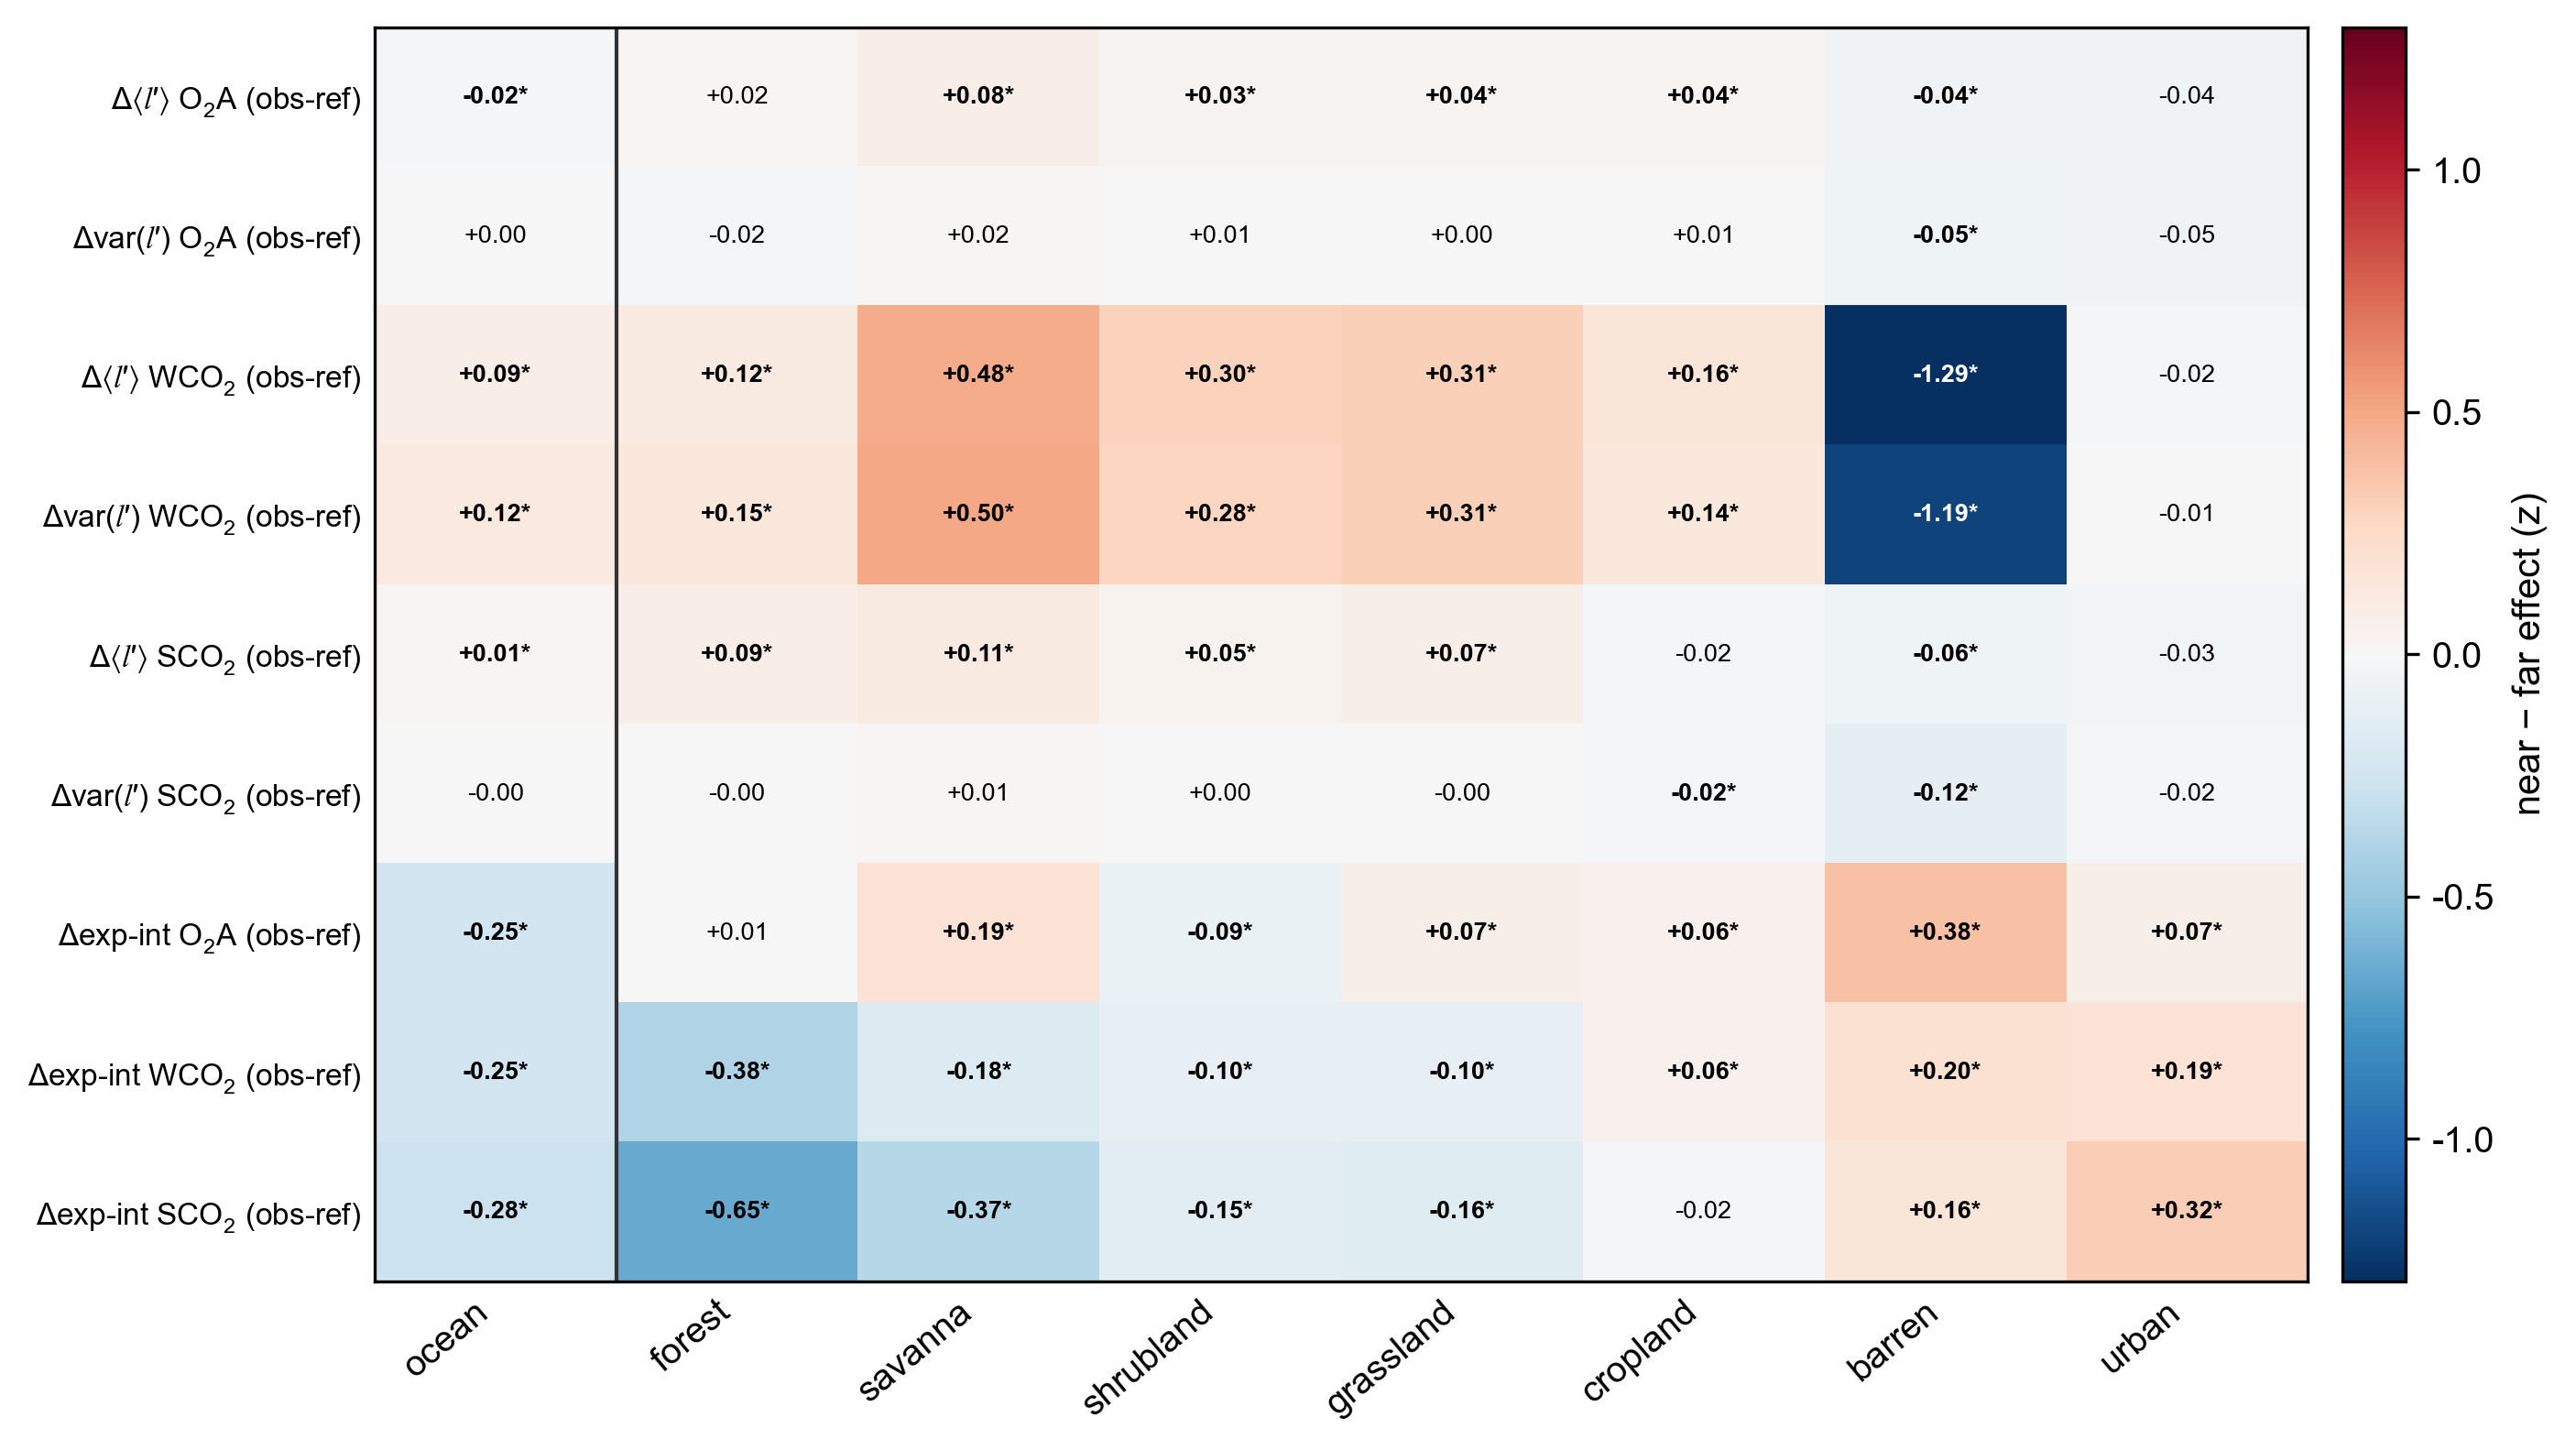
\includegraphics[width=\textwidth]{figures/fig04_landclass_effect_heatmap.png}
\caption{Surface-stratified near-cloud spectral response of effect size (Eq. \ref{eq:effect-size}; near-cloud 0–5 km minus far-cloud 20–50 km, in far-field standard deviations) of the reference-corrected path-length features for ocean and for each MCD12C1 land-cover class. Quality-flag-0, snow-free soundings; per-sounding references use the surface-specific clear-sky radii of the production targets (ocean beyond 5 km, land beyond 15 km); asterisks mark effects exceeding their analytic 95 \% confidence interval. ⟨$l′$⟩ and var($l'$) are the fitted mean and variance of the relative photon path (the cumulants k1, k2 of Sect. 3.2). Reference and quality-flag sensitivity variants: Appendix B.}
\label{fig:land_type_features}
\end{figure}




\begin{figure}[t]
\centering
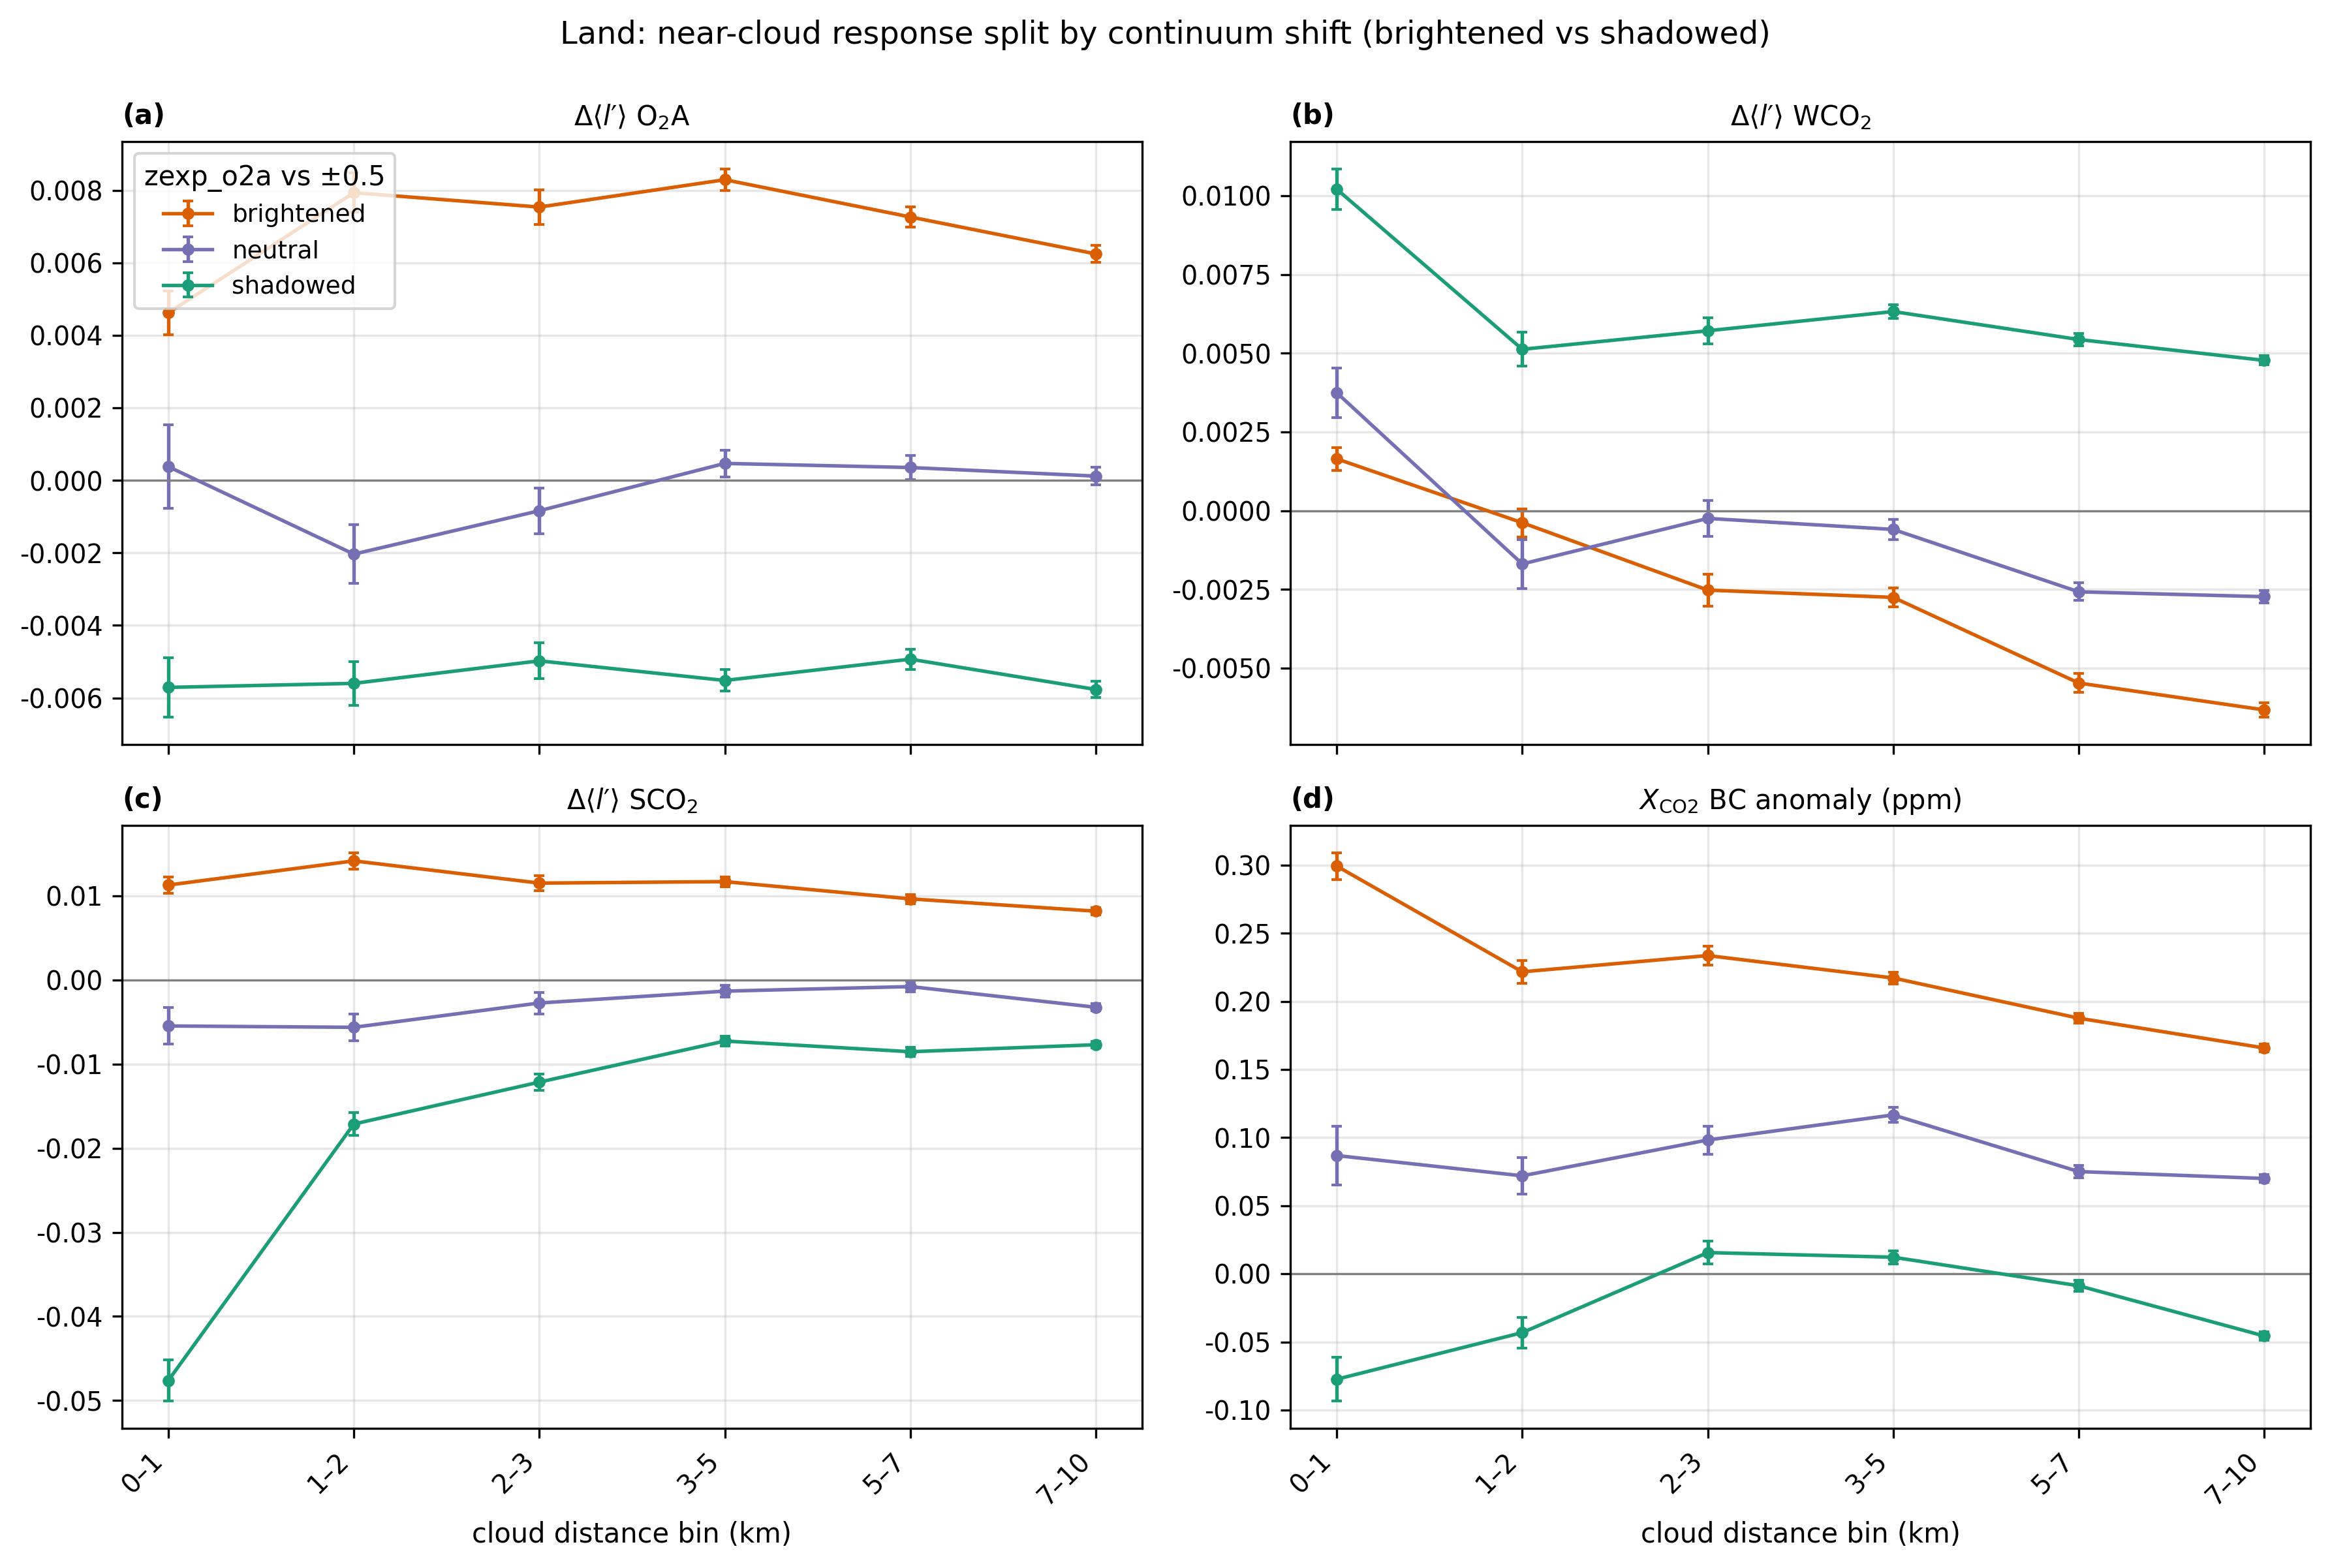
\includegraphics[width=0.8\textwidth]{figures/fig05_shadow_brightening_land.png}
\caption{Shadowing versus brightening. Near-cloud land footprints split by the sign of the \ce{O2}A continuum-reflectance departure from the clear-sky reference (exp-intercept low: cloud shadowing; high: side illumination/brightening), with each branch's \xco anomaly and band-resolved $\Delta$ ⟨$l′$⟩ response. (A single-overpass illustration against Aqua-MODIS true-colour imagery: Appendix G, Fig. G1.)}
\label{fig:shadow-brightening}
\end{figure}




\FloatBarrier